\chapter{Overcoming Grobner Basis Complexity for Abstraction} \label{ch:improv}

Computing a \Grobner basis is prohibitively expensive for large circuits. 
%The worst-case complexity of computing $GB(J + J_0)$
%in $\Fq[x_1, \dots, x_d]$ is known to be bounded by $q^{O(d)}$
%\cite{gao:gf-gb-ms}, which is prohibitive over large
%fields. 
The approach from the last 
chapter is limited only to small circuits, with data-paths no larger than 
$40$-bits. 
A full \Grobner basis computation results in numerous polynomials, but
the abstraction approach ``searches'' for only one
polynomial ($Z + \G(A)$) in the basis. This motivates an investigation into
whether it is possible to {\it  guide a sequence of $Spoly(f,
  g)\xrightarrow{J+J_0}_+ r$  computations} to arrive at the desired
word-level polynomial. This chapter describes this 
{\it smaller subset} of computations, which are derived from a \Grobner basis 
analysis, to find the word-level polynomial of the function performed by a 
given circuit. The improved approach can abstract canonical word-level 
representations of circuits up to $571$ bits, 
corresponding to the largest NIST-specified ECC standard. 

\section{Improving the Abstraction Approach}
Consider the word-level abstraction problem formulation from 
Chapter \ref{ch:abstract}. $J$ is the ideal 
generated by all polynomials derived from the circuit implementation and 
$J_0$ is the ideal of all the vanishing polynomials of 
every variable in the ring. 
The computation of the reduced \Grobner basis of $J+J_0$ over $\Fq$ 
has the following known complexity\cite{gao:gf-gb-ms}:

\begin{Theorem}
Let $J+J_0 = \langle f_1, \dots, f_s, ~x_1^q - x_1, \dots, x_d^q -
x_d\rangle \subset \Fq [x_1, \dots, x_d]$ be an ideal. The time and
space complexity of Buchberger's algorithm to compute a \Grobner
basis of $J+J_0$ is bounded by $q^{O(d)}$.
\end{Theorem}

In our case $q = 2^k$, and when $k$ and $d$ are large, this complexity 
makes abstraction infeasible.

Recall that Buchberger's algorithm \cite{buchberger_thesis} for 
computing \Grobner bases depends on the computation of an $S$-polynomial, 
which is then reduced by all the polynomials in the basis. 

\begin{equation}
Spoly(f_{i}, f_{j}) \stackrel{G'}{\textstyle\longrightarrow}_+r \nonumber
\end{equation}
where
\begin{eqnarray}
Spoly(f,g)=\frac{L}{lt(f)}\cdot f - \frac{L}{lt(g)}\cdot g \nonumber \\ 
\nonumber \\
L=lcm(lt(f),lt(g)) \nonumber
\end{eqnarray}

A new polynomial is added to the basis when the remainder of the $Spoly$
reduction, $r$, is non-zero.

Notice that our approach searches
for only one polynomial $f_\Func:Z+\Func(A_1,\dots,A_n)$, and it does
by computing the entire reduced \Grobner basis, $G=\{g_1,\dots,g_m\}$ and
finding $f_\Func\in \{g_1,\dots,g_m\}$.
This motivates us to
investigate whether it's possible to {\it  guide a sequence of 
$Spoly(f,g)\xrightarrow{J+J_0}_+ r$  computations} to arrive at the desired
word-level polynomial, without considering other polynomials in the
generating set. 

Numerous improvements have been introduced to improve the efficiency of 
Buchberger's algorithm. One of these is the product criterion, the results
of which we exploit for our approach.

\begin{Lemma}
\label{lemma:prodcriteria}
[Product Criterion \cite{productc:1979}] Let $\mathbb{F}$ be any
field, and $f, g \in \mathbb{F}[x_1,\cdots,x_d]$ be polynomials. If
the equality $lm(f) \cdot lm(g) = LCM(lm(f), lm(g))$ holds, then
$Spoly(f,g)\stackrel{G}{\textstyle\longrightarrow}_+ 0.$ 
\end{Lemma}

The above result states that when the leading monomials of $f, g$ are
relatively prime then 
$Spoly(f, g)$ always reduces to 0 modulo $G$. In this case,
$Spoly(f, g)$ need not be considered in Buchberger's algorithm, and thus
the computation is avoided. 
Recall that in the Abstraction Term Order (Definition \ref{def:ato}),
we have ``circuit variables $x_1, \dots, x_d$'' $>$ ``word-level output''
$>$ ``word-level inputs'', where the
relative ordering among  $x_1, \dots, x_d$ is not important. This ordering
is now further refined to exploit the product criteria.

Given an acyclic combinational circuit, an ordering can be applied to the 
bit-level variables, $\{x_1,\dots,x_d\} \in \F_2$, 
based on their topological position in the circuit. In a {\it reverse topological
ordering}, the output variable of the gate will always come earlier in the
ordering than any of its input variables.
%This is denoted {\bf topological ordering}.

%\begin{Definition}
%Given a Boolean combinational circuit, let the topological location of the 
%bit-level variable $x$, denoted as $TL(x)$, be the 
%maximum number of Boolean logic gates that any path from any input must 
%pass to reach the variable. Then the variable ordering 
%\begin{equation}
%x>y : TL(x)<TL(y) 
%\end{equation}
%is denoted {\bf topological ordering}. Likewise, the ordering 
%\begin{equation}
%x>y : TL(x)>TL(y) 
%\end{equation}
%is a {\bf reverse topological ordering}.
%\label{def:topord}
%\end{Definition}
%\begin{Example}
%Consider the combinational circuit shown in Figure \ref{fig:topo}.
%This circuit has two bit-level inputs
%$a$ and $b$, intermediate variable $c$; and output $z$.

%\begin{figure}[H]
%\centerline{
%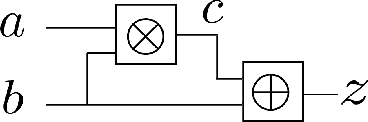
\includegraphics[scale=0.6]{./figures/topoExample.png}
%}
%\caption{Boolean combinational circuit.}
%\label{fig:topo}
%\end{figure}

%Then:
%\begin{eqnarray}
%TL(a)=0 \nonumber \\
%TL(b)=0 \nonumber \\
%TL(c)=1 \nonumber \\
%TL(z)=2 \nonumber
%\end{eqnarray}

%Thus, $a > b > c > z$ is a topological ordering. 
%Since $TL(a)=TL(b)$, $b > a > c > z$ is also a topological 
%ordering. 

%Likewise, $z > c > a > b$ and $z > c > b > a$ are considered reverse
%topological orderings.
%\end{Example}


\begin{Definition}
\label{def:rato}
{\bf Refined Abstraction Term Order (RATO) $>_r$:} 
%Starting from the primary
%outputs of the circuit $C$, perform a reverse topological traversal
%toward the primary inputs. Order each variable of the circuit
%according to its reverse topological level: i.e. $x_i > x_j$ if $x_i$
%appears earlier in the reverse topological order.
Given a circuit $C$, apply a reverse topological ordering to the bit-level
variables $\{x_1, \dots, x_d\}$.
Then, impose a lex term
order $>_r$ on $\Fq[x_1, \dots, x_d, Z, A_1, \dots, A_n]$ with ``circuit 
variables ordered reverse topologically'' $>$ 
``output word-level variable'' $>$ ``input word-level variables''. 
%This term order $>_r$ is called the {\bf refined abstraction term order (RATO)}.
\end{Definition}

Let $F$ be the set of polynomials which generate $J$, i.e. $J=<F>$. 
When RATO is applied, 
we find that all 
{\it bit-level circuit constraint
polynomials} in $F$ have leading terms that are relatively prime to each 
other. Since we are using a
reverse topological variable ordering with lex term ordering, these 
polynomials are in the 
form of $f_i = x_i + \text{tail}(f_i)$, where $x_i$ is the output of a gate $f_i$, 
and thus the following
proposition from {\it Lv's} work \cite{lv:phd} can be applied.

\begin{Proposition} \label{prop:top-order}
Let $C$ be any arbitrary combinational circuit. Let $\{x_1, \dots,
x_d\}$ denote the set of all variables (signals) in the circuit,
i.e. the primary input, intermediate and primary output
variables. Perform a {\bf reverse topological traversal} of the
circuit and order the variables such that $x_i > x_j$ if $x_i$ appears
earlier in the reverse topological order. Impose a lex term order to
represent the Boolean expression for each gate as a polynomial $f_i$;
then $f_i = x_i + \text{tail}(f_i)$. Then the set of all polynomials
$\{f_1, \dots, f_s\}$ forms a Gr\"obner basis, as $lt(f_i)$ and $
lt(f_j)$ for $i\neq j$ are relatively prime. 
\end{Proposition}

\begin{Example}
Consider the $2$-bit multiplier from Example 
\ref{exp:finalMul2Bit}. With RATO applied, the bit-level circuit constraint
polynomials in $F$, where $J=<F>$, are:
\begin{eqnarray}
		f_1:c_0+a_0 \cdot b_0 \nonumber \\
		f_2:c_1+a_0 \cdot b_1 \nonumber \\
		f_3:c_2+a_1 \cdot b_0 \nonumber \\
		f_4:c_3+a_1 \cdot b_1 \nonumber \\
		f_5:r_0+c_1 + c_2		\nonumber \\
		f_6:z_0+c_0 + c_3	\nonumber	\\
		f_7:z_1+r_0 + c_3	\nonumber	
\end{eqnarray}
The leading terms of $f_1,\dots,f_7$ are relatively prime to each other.
\label{exp:2bitmulrato}
\end{Example}

Let $F_0$ be the set of polynomials which generate $J_0$, i.e. $J_0=<F_0>$.
In $F\cup F_0$, for every polynomial $f_i = x_i + \text{tail}(f_i)$ 
in $F$ there is a vanishing polynomial $v_i = x_i^2+x_i$ in $F_0$; 
$f_i$ and $v_i$ have leading terms which are not relatively prime.
In this case, 
\cite{lv:phd} shows that $Spoly(x_i+\text{tail}(f_i), x_i^{2^k}-x_i)
\stackrel{J,J_0}{\longrightarrow}_+ r$ always produces $r=0$, and thus can
be excluded from the \Grobner basis computation.

\begin{Theorem}
\label{thm:lvcontrib}
Let $q = 2^k$, and let $\Fq[x_1, \ldots, x_d]$ be a ring on
which we have a reverse topological lex order. Let $I$ be a subset of $\{1,
\ldots, d\}$. For all $i \in I$, let $f_i = x_i +P_i$ (where $P_i =
\text{tail}(f_i)$) such that  all indeterminates $x_j$  that appear in
$P_i$ satisfy $x_i > x_j$.  Then the set $G = \{f_i :  i  \in I\} \cup
\{x_1^q-x_1, \ldots, x_d^q-x_d\}$ is a Gr\"obner basis. 
\end{Theorem}

The proof is given in \cite{lv:phd} and is reproduced here:

\begin{Proof}
Given a system of polynomials derived from a circuit over 
$\Fq[x_1, \ldots, x_d]$, where $\{x_1,\dots,x_d\}$ are bit-level variables.
Apply a reverse topological lex ordering to $\{x_1,\dots,x_d\}$. 
Let $x_i$ be the output of a Boolean logic gate for some $1\leq i \leq d$.
Let $f = x_i + P_i$ be the polynomial derived from this logic gate and
$g = x_i^q-x_i$ be vanishing polynomial of $x_i$.
Then $Spoly(f,g)=
x_i^{q-1} f - g = x_i^{q-1}P_i + x_i$. In what follows, it is important
to note that the indeterminates appearing in $P_i$ are all less than
$x_i$ over the given ordering.  

First,  $x_i^{q-1}P_i +x_i - x_i^{q-2}P_i(x_i+P_i)=x_i^{q-2}P_i^2 +x_i,$ 
which shows that 
$x_i^{q-1}P_i +x_i \stackrel{x_i+P_i}{\longrightarrow}  x_i^{q-2}P_i^2
+x_i.$  

Next, $x_i^{q-2}P_i^2 + x_i - x_i^{q-3}P_i^2(x_i+P_i)=
x_i^{q-3}P_i^3+ x_i.$ Continuing in this fashion, we get $x_iP_i^{q-1}
+x_i-P_i^{q-1}(x_i+P_i) = x_i + P_i^q,$ and finally 
$x_i+P_i^q -(x_i+P_i) = P_i^q-P_i.$ Hence, 
$$x_i^{q-1}P_i +x_i \stackrel{x_i+P_i}{\longrightarrow} x_i^{q-2}P_i^2
+x_i \stackrel{x_i+P_i}{\longrightarrow} x_i^{q-3}
+x_i \stackrel{x_i+P_i}{\longrightarrow} \cdots$$
$$\cdots \stackrel{x_i+P_i}{\longrightarrow}
P_i^q+x_i\stackrel{x_i+P_i}{\longrightarrow} P_i^q-P_i.$$ 


Over the finite field $\mathbb{F}_{q}$, $P_i^q-P_i$ is a vanishing
polynomial. Therefore, $P_i^q-P_i \in I(V(J_0))= \langle
x_1^q-x_1, \ldots, x_d^q-x_d\rangle$. Due to the product criterion
(Lemma \ref{lemma:prodcriteria}), $G_0=\{x_1^q-x_1, \ldots, x_d^q-x_d\}$ is
Gr\"obner basis. Therefore 
$P_i^q-P_i \stackrel{G_0}\rightarrow_+ 0$. 
\end{Proof}

Due to RATO, there exists a polynomial $f_{z_i}\in F$ which is the 
polynomial derived from a Boolean logic gate, where $z_i$ is the first 
variable in the ordering for some $0\leq i <k$. That is, $f_{z_i}: z_i+\text{tail}(f_{z_i})$.
\begin{Proposition}
Over RATO, the polynomial pair $(f_Z, f_{z_i})$ is the only critical pair
at the start of the \Grobner basis computation of $J+J_0$, where 
$f_{z_i}$ is the polynomial derived from the gate
\end{Proposition}
\begin{Proof}
Due to Theorem \ref{thm:lvcontrib} and the product criterion, 
a critical pair must come from a word level designation polynomial, 
$\{f_Z,f_{A_1},\dots,f_{A_n}\}$, and a polynomial derived from a Boolean logic
gate. The leading terms of the polynomials $\{f_{A_1},\dots,f_{A_n}\}$ are 
bit-level inputs to the circuit and thus are not the outputs of any gate.
Thus, the only critical pair if $f_Z$ and $f_{z_i}$, where $z_i$ is the first
variable in the ordering and is thus the leading monomial of $f_Z$.
\end{Proof}
%Thus, we are left with only a few options for an $Spoly$ at the  
%beginning of a \Grobner basis computation of $J+J_0$ with abstraction order
%$>$. Consider the {\it word-level designation polynomials} 
%$\{f_{Z},f_{A_1},\dots,f_{A_n}\}$ in $J$. Since all word-level variables 
%are found last in abstraction order, the leading monomial of each of these
%polynomials is some bit-level $x_d$. Thus there is a vanishing polynomial
%$x_d^2+x_d$ with the same leading monomial. Take $f_Z$ for example:

%\begin{eqnarray}
%f_{Z}: z_{0}+z_{1}\cdot \alpha,\cdots,{z_{k-1}}\cdot \alpha^{k-1}+Z \nonumber \\
%f_{v}: z_0^2+z
%\end{eqnarray}


%Thus, there are no valid $S$-polynomials which can be generated using
%the set $\{$bit-level constraints $\in J$,  $J_0\}$.
%So a valid $S$-polynomials must be generated using at least 
%one {\it word-level designation polynomial}, $f_Z,f_{A_1},\dots,f_{A_n}$.
%Consider the output word-level designation polynomial $f_Z$:
%\begin{equation}
%f_Z: Z+z_0+z_1\alpha+\dots+z_{k-1}\alpha^{k-1}
%\end{equation}
%Since all word-level variables 
%are found last in RATO, the leading monomial of $f_Z$ 
%has to be a bit-level output variable, $z_i$, for some $0\leq i < k$. 
%Since $z_i$ is the output of a Boolean logic gate, there 
%exists a polynomial $f_{z_i} \in J$ with $z_i$ as the leading monomial, 
%$f_{z_i}:z_i + \text{tail}(f_{z_i})$. $Spoly(f_Z,f_{z_i})$ is 
%a valid $S$-polynomial, and it has
%some interesting properties.

Thus, the first computation of the \Grobner basis is guaranteed to be 
$Spoly(f_Z,f_{z_i})\xrightarrow{F,F_0}_+ r$.
This computation has the following interesting property.

\begin{Proposition} \label{prop:reduce}
Normalize $f_Z$, i.e. $f_Z$=$f_Z/LC(f_Z)$. Then
\begin{eqnarray}
Spoly(f_Z,f_{z_i})\xrightarrow{F,F_0}_+ r & \text{is equivalent to} &
f_Z\xrightarrow{F-\{f_Z\},F_0} + r
\end{eqnarray}
\end{Proposition}

%% \begin{Proposition} \label{prop:reduce}
%% Let $C$ be any arbitrary combinational circuit with $k$-bit inputs 
%% $A_1,\dots,A_n$ and $k$-bit output $Z$. Model the circuit as a system of 
%% polynomials as described earlier.
%% Let $f_Z$ be the word-level 
%% designation polynomial $Z+z_0+z_1\alpha+\dots+z_{k-1}\alpha^{k-1}$. By
%% applying RATO, the leading monomial of $f_Z$ will be $z_i$ for some
%% $0\leq i < k$.
%% There exists a polynomial $f_{z_i}$ in the form of $z_i+\text{tail}$, 
%% which is the polynomial representation of the 
%% Boolean gate with output $z_i$.
%% %Then if $f_Z$ and $f_i$ is first minimized, i.e. $f_Z$=$f_Z/LC(f_Z)$, 
%% Then 
%% \begin{equation}
%% Spoly(f_Z,f_{z_i})\stackrel{J,J_0}{\longrightarrow}_+ r
%% \end{equation}
%% is equivalent to
%% \begin{equation}
%% %f_Z\stackrel{J-\{f_Z\},J_0}{\longrightarrow}_+ r
%% f_Z\xrightarrow{J-\{f_Z\},J_0} + r
%% \end{equation}
%% \end{Proposition}

\begin{Proof}
Assuming both $f_{z_i}$ and $f_Z$ are minimized, i.e. 
$LC(f_{z_i})=LC(f_Z)=1$, 
they are both in the form $z_i+P$ for some polynomial $P$.
Let $f=z_i+P_f$ and $g=z_i+P_g$ represent $f_{z_i}$ and $f_Z$ respectively.

(i) For $Spoly(f,g)$
\begin{equation}
L=LCM(LT(f),LT(g))=LM(f)=LM(g)=z_i
\end{equation}
so
\begin{eqnarray}
Spoly(f,g)&=&\frac{L}{lt(f)}\cdot f - \frac{L}{lt(g)}\cdot g \nonumber \\
&=&\frac{z_i}{z_i}\cdot f - \frac{z_i}{z_i}\cdot g \nonumber \\
&=&f + g \nonumber
\end{eqnarray}
Thus 
$Spoly(f_Z,f_{z_i})\stackrel{F,F_0}{\longrightarrow}_+ r$
is equivalent to 
$f+g\stackrel{F,F_0}{\longrightarrow}_+ r$.

(ii) For $f_Z\xrightarrow{F-\{f_Z\},F_0} + r$, since the leading term 
of $f_Z$ is $z_i$, the only polynomial in the set $\{F-\{f_Z\},F_0\}$
which can perform the first division is $f_{z_i}$. 
Again, denote $f_Z$ as $f$ and $f_{z_i}$ 
as $g$. According to the reduction algorithm, the remainder $r$ of 
$f\stackrel{g}{\longrightarrow}_+ r$ is:
\begin{eqnarray}
r &=& f-lt(f)/lt(g) \cdot g \nonumber \\
  &=& f-z_i/z_i \cdot g \nonumber \\
  &=& f-g \nonumber \\
  &=& f+g
\end{eqnarray}
Thus 
$f_Z\xrightarrow{F-\{f_Z\},F_0} + r$
is equivalent to 
$(f+g)\xrightarrow{F-\{f_Z\},F_0} + r$

(iii) Consider $(f+g)\xrightarrow{F,F_0} + r$. $f=z_i+P_f$ and 
$g=z_i+P_g$. So $f+g=2z_i+P_g+P_f=P_g+P_f$ no longer contains $z_i$ as the 
leading monomial. As a consequence of RATO, as 
reduction proceeds the remainder will never again contain 
$z_i$ since $z_i$ is the first variable in the ordering. 
Since the leading monomial of $f_Z$ is $z_i$, $f_Z$ will never be 
used for reduction. Therefore 
$(f+g)\xrightarrow{F,F_0}+ r$
is equivalent to 
$(f+g)\xrightarrow{F-\{f_Z\},F_0}+ r$

Thus, 
$Spoly(f_Z,f_{z_i})\stackrel{F,F_0}{\longrightarrow}_+ r$
is equivalent to
$f_Z\xrightarrow{F-\{f_Z\},F_0}_+ r$
\end{Proof}

%Due to the reverse-topological abstraction order, 
%since there is a $x_i + \text{tail}$ for every $x_i \in \{x_1,\dots,x_d\}$ 
%except the bit level inputs $a_0,\dots,a_k$,
%$f_Z\xrightarrow{J-\{f_Z\},J_0}+ r$ can only contain the bit-level
%inputs $a_0,\dots,a_k$, the word level inputs $A_1,\dots,A_n$, and the 
%word-level output $Z$. 
Thus, $f_Z\xrightarrow{F-\{f_Z\},F_0}_+ r$ is the first computational step 
of the abstraction.
The polynomial remainder $r$
will {\it not} contain any bit-level variable corresponding to the
output of any gate in the design;  i.e. primary output bits and
intermediate variables of the circuit do not appear in $r$. To prove
this, assume that a non-primary-input variable $x_j$ appears in a
monomial term $m_j$ in $r$. Since there always exists a polynomial
$f_j$ such that $f_j = x_j + \text{tail}(f_j)$, $lt(f_j)$
divides monomial $m_j$ and $m_j$ can be canceled. Therefore, all
such terms $m_j$ with non-primary-input bit-level variables can be
eliminated.  

Two cases need to be considered: 
\begin{enumerate}
\item Remainder $r$ only contains word-level variables:
  word-level output $Z$ and the word-level 
  inputs $A_1,\dots,A_n$. 
  Since RATO is lex with $Z > \{A_1,\dots,A_n\}$, the remainder $r$
  is the desired canonical polynomial representation,
  $Z + \Func(A_1,\dots,A_n)$.
\item Remainder $r$ contains both the bit-level primary
  input variables, as well as the word-level
  variables.  
\end{enumerate}

%We've found that for bug-free Galois field
%arithmetic circuits,
%when we compute $Spoly(f_{Z},f_{z_i})\stackrel{J,J_0}{\longrightarrow}_+ r$, 
%$r$ only contains variables in $A_1,\dots,A_n,Z$ and is thus {\bf canonical, 
%word-level polynomial } in the form of 
%$Z+\Func(A_1,\dots,A_n)$.

\begin{Example}
\label{exp:absGood}
Again consider the $2$-bit multiplier from Example 
\ref{exp:2bitmulrato}.
RATO for this example is
\begin{equation}
z_1 > z_0 > r_0 > c_0 > c_1 > c_2 > c_3 > a_0 > a_1 > b_0 > b_1 > Z > A > B 
\end{equation}
$F+F_0$ with RATO applied is:
\begin{eqnarray}
 \left .  
	\begin{aligned}
		f_1:c_0+a_0 \cdot b_0  \\
		f_2:c_1+a_0 \cdot b_1  \\
		f_3:c_2+a_1 \cdot b_0  \\
		f_4:c_3+a_1 \cdot b_1  \\
		f_5:r_0+c_1 + c_2		\\
		f_6:z_0+c_0 + c_3		\\
		f_7:z_1+r_0 + c_3		
	\end{aligned} 
 \ \right\}
 &\qquad&  {\it  \text{Bit-level circuit constraints} ~(\subset J)} \nonumber \\
 \left . 
	\begin{aligned}
		f_{A}:a_0+a_1\cdot \alpha + A  \\ 
		f_{B}:b_0+b_1\cdot \alpha + B \\ 
		f_{Z}:z_1\cdot \alpha + z_0 + Z  
	\end{aligned} 
 \right\}
 &\qquad&  {\it  \text{Word-level designation} ~(\subset J)} \nonumber \\
  \left . 
	\begin{aligned}
		a_0^2-a_0, ~a_1^2-a_1,~b_0^2-b_0, ~b_1^2-b_1   \\ 
		c_0^2-c_0, ~c_1^2-c_1,~c_2^2-c_2, ~c_3^2-c_3  \\ 
		r_0^2-r_0, ~z_0^2-z_0,~z_1^2-z_1    \\ 
		A^4-A, ~B^4-B ,~Z^4-Z		  
	\end{aligned} 
 \right\}
 &\qquad&  {\it \text{vanishing polynomials} (J_0)} \nonumber
\end{eqnarray}
Notice that the leading monomial of $f_Z$ is $z_1$, which is also the leading monomial 
of $f_7$.
Minimize $f_Z$, 
$f_{Zmin}=f_Z/\alpha = z_1 +z_0\cdot(\alpha+1)+Z\cdot(\alpha+1)$.
By computing the $S$-polynomial of $f_{Zmin}$ and $f_7$:
\begin{equation}
Spoly(f_{Zmin},f_{7})\stackrel{F,F_0}{\longrightarrow}_+ r \nonumber
\end{equation}
the remainder $r$ is $Z+A\cdot B$.

Likewise, if we reduce $f_{Z}$ by $F-\{f_Z\},F_0$, that is reduce it by all
generators in $J+J_0$ except $f_Z$:
\begin{equation}
f_{Z}\xrightarrow{F-\{f_Z\},F_0} + r \nonumber
\end{equation}
the remainder $r$ is $Z+A\cdot B$. 
\end{Example}

%As this abstraction process can be computed as a reduction procedure, we
%created a highly efficient reduction tool over $Fkk$. Using this tool, we
%are able to abstract word-level polynomial representations for bug-free 
%circuits up
%to $407$-bits in size. When applied to buggy circuits, however, 
%approach yields a polynomial which includes bit-level input variables.

\begin{Example}\label{ex:improve1}
Now consider a $2$-bit multiplier which has a {\bf bug}.
The output lines, $z_0$ and $z_1$, have been swapped, as shown in 
Figure \ref{fig:2bitmulbug} below:

\begin{figure}[H]
\centerline{
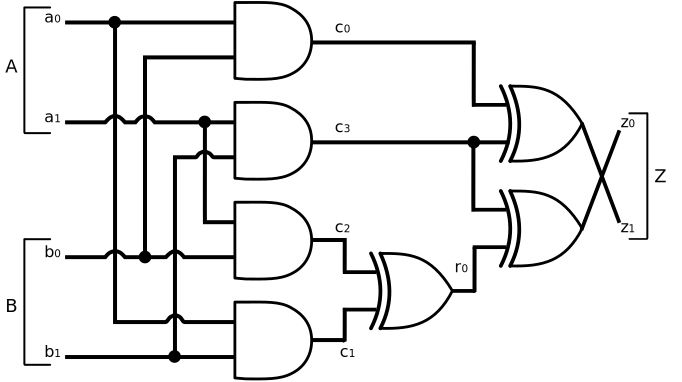
\includegraphics[scale=0.4]{./figures/2bitmasmultBUGswap}
}
\caption{ A buggy 2-bit multiplier over ${\mathbb{F}}(2^2)$.}
\label{fig:2bitmulbug}
\end{figure}

The polynomials in $F+F_0$ are the same as in Example \ref{exp:absGood} 
except for the following changes:
\begin{eqnarray}
f_6:z_1+c_0 + c_3	\nonumber	\\
f_7:z_0+r_0 + c_3	\nonumber	\\
f_Z:z_1 + z_0\cdot \alpha + Z  \nonumber	
\end{eqnarray}

$f_Z$ has common leading terms with $f_6$. Computing 
\begin{equation}
Spoly(f_Z,f_{6})\stackrel{F,F_0}{\longrightarrow}_+ r \nonumber
\end{equation}
gives remainder $r: a_1\cdot b_1 \alpha + a_1\cdot B \alpha + b_1 \cdot A \alpha + Z + A\cdot B$, which is the same result as computing
$f_Z\xrightarrow{F-\{f_Z\},F_0}_+ r$
\label{exp:2bitbugmulex}
\end{Example}

%%%%%%%%%%%%%%%%%%%%%%F4-STYLE REDUCTION%%%%%%%%%%%%%%%%%%%%%%%%%%%%%

\section{Improving Polynomial Division using $F4$-style Reduction}

The most intensive computational step in our proposed improvement 
is that of polynomial division $f_Z \xrightarrow{F-\{f_Z\},F_0}_+ r$. 
When the circuit $C$ is very large, the polynomial set
$\{F-\{f_Z\},F_0\}$ also becomes extremely large. This division
procedure then becomes the bottleneck in our abstraction approach.  
In principle, this reduction can be performed using contemporary
computer-algebra systems --- {\it e.g.},  the {\sc Singular}
\cite{DGPS} tool, which is widely used within the verification
community \cite{wienand:cav08} \cite{wedler:date11}
\cite{lv:date2012}. In our work, we have also performed experiments 
with {\sc Singular}. However, as in any ``general-purpose''
computer algebra tool, the data-structures are not specifically
optimized for circuit verification problems. Moreover, {\sc
  Singular} also limits the number of variables ($d$) that it can
accommodate in the system to $d < 32767$; this limits its
application to large circuits. Recent symbolic computation techniques \cite{lv:phd}
have shown improvements from employing the concept of $F4$-style 
polynomial reduction \cite{f4}.
Therefore, to further improve our
approach, we exploit this relatively recent concept, 
which implements polynomial division
using row-reductions on a matrix, to develop a custom
verification tool to perform this reduction
efficiently.

$Faug\grave{e}re$'s $F4$ approach \cite{f4} presents a new algorithm to
compute a Gr\"obner basis. It uses the same mathematical principles as
Buchberger's algorithm. However, instead of computing and reducing one 
$S$-polynomial at a time, it computes many $S$-polynomials in one
step and reduces them simultaneously using sparse linear algebra on a
matrix (triangulation). We can use this efficient reduction technique
to perform our reduction, $f_Z \xrightarrow{F-\{f_Z\},F_0}_+ r$, by 
representing and solving it on a matrix.
First, let us consider the following example that demonstrates the
main concepts behind the reduction approach of $F4$. 

\begin{Example}
{\it
Consider the {\it lex} term order with $x>y>z$ on the ring
${\mathbb{Q}}[x, y, z]$.  Given $F = \{f_1 = 2x^2 + y, f_2 = 3xy^2
-xy, f_3 = 4y^3 -1\}$, consider one step of Buchberger's algorithm:
$S(f_1, f_2) \xrightarrow{f_1, f_2, f_3}_+r$. We have, $Spoly(f_1,
f_2) = \frac{1}{3}x^2y + \frac{1}{2}y^3 = f_4$. The reduction
$Spoly(f_1, f_2)\stackrel{f_1, f_2, f_3}{\longrightarrow}_+
(-\frac{1}{6}y^2 + \frac{1}{8})$ is done as follows: 
Since $lt(f_1) ~|~ lt(f_4), ~f_4 \xrightarrow{f_1} h$ is computed as:
\[
h = f_4 - {{lt(f_4)} \over {lt(f_1)}} f_1 = f_4 - \frac{1}{6}y f_1 =
\frac{1}{2}y^3 - \frac{1}{6}y^2; 
\]
Now $lt(f_2)$ does not divide any term in $h$, but $lt(f_3) ~|~ lt(h)$,
so $f \xrightarrow{f_3} r$:
\[
r = h - {{lt(h)} \over {lt(f_3)}} f_3 =  \frac{1}{2}y^3 - \frac{1}{6}y^2 -
\frac{1}{8}f_3 = -\frac{1}{6}y^2 + \frac{1}{8} 
\]

This reduction procedure can also be simulated on a matrix using
Gaussian elimination. 
%Matrix triangulation can also be used for this purpose. 
The reduction above requires the computation of $\frac{1}{6}y f_1$ and 
$\frac{1}{8}f_3$. Ignoring the coefficients $\frac{1}{6},
\frac{1}{8}$, 
we can generate all the monomials  required in the reduction process: 
i.e.  monomials of $f_4, yf_1, f_3$, and setup the problem of
cancellation of terms as Gaussian elimination on a matrix. Monomials
of $f_4, yf_1, f_3$ are, respectively, $\{x^2y, y^3\}, \{x^2y, y^2\}, \{y^3, 1\}$.
Let the rows of a matrix $M$ correspond to polynomials $\left[ f_4,
  yf_1, f_3   \right]$, and columns correspond to all the monomials
(in {\it lex} order) $\left[x^2y, y^3, y^2,  1 \right]$. Then the
matrix $M$ shows the representation of these polynomials where
the entry $M(i, j)$ is the coefficient of monomial of column $j$
present in the polynomial of row $i$.

\[
M = \bordermatrix{
~ & x^2y & y^3 & y^2 & 1\cr
f_4 & \frac{1}{3} & \frac{1}{2} & 0 & 0 \cr
yf_1 & 2 &0 & 1 & 0 \cr
f_3 & 0 & 4 & 0 & -1 \cr
}
\]

Now, reducing $M$ to a row echelon form using Gaussian elimination gives:
\[
M = \bordermatrix{
~ & x^2y & y^3 & y^2 & 1\cr
f_4 & \frac{1}{3} & \frac{1}{2} & 0 & 0 \cr 
h = f_4 - \frac{1}{6}yf_1 & 0 &\frac{1}{3}  & -\frac{1}{6} & 0 \cr 
r = h - \frac{1}{8}f_3 & 0 & 0 & -\frac{1}{6} & \frac{1}{8} \cr 
}
\]

The last row $(0, 0, -\frac{1}{6}, \frac{1}{8})$ accounts for
polynomial $-\frac{1}{6}y^2 + \frac{1}{8}y$ which is equal to the
reduction result $r$ obtained before. 
}
\end{Example}

This approach generates all the monomial terms that are required
in the division process, 
%i.e. $\frac{lm(f_i)}{lm(f_j)} f_j$, 
and the coefficients required for cancellation of terms are accounted
for by elementary row reductions in the subsequent Gaussian elimination. 
Based on the above concepts, a matrix can be constructed for our
problem: $f_Z \xrightarrow{F-\{f_Z\},F_0}+r$. 

\begin{Definition}
Let $L = \left [f_1, \dots, f_m \right]$ be a list of $m$ polynomials. Let
$M_L$ be an ordered list of monomials of elements of $L$ and let $n$
be the number of elements in $M_L$. Define $M$ as the $m \times n$
matrix which associates the polynomials of $L$ to rows and monomials
of $M_L$ to columns. Entry in row $i$, column $j$ is the coefficient of the
$j^{th}$ element of $M_L$ in $f_i$. 
\end{Definition}

\begin{algorithm}[hbt]
\SetAlgoNoLine

 \KwIn{$f_Z, \{F-\{f_Z\},F_0\}$ as $\{f_1,\dots,f_s\}$, RATO $>_r$ } %with $f_{1}>f_{2}>\dots>f_{s}$. }
 \KwOut{Remainder $r$ of $f_Z \xrightarrow{f_1,\dots,f_s}_+r$}
  %%%%%%%%%%%%%%%%%%%%
        \CommentSty{/*$L=$ set of polynomials, rows of $M$*/\;}
        L:=\{$f_Z$\} \;{}
%        \CommentSty{/*The index of polynomials in $L$*/\;}
%       \CommentSty{/*Initial remainder $r$ is set as $f$*/\;}
%       r:=f\;
        \CommentSty{/*$M_{L} = $ the set of monomials, columns of $M$ */\;}
        $M_{L}$:=\{ monomials of f\} \;{}
%       \CommentSty{/*Let $Done$ be the set of monomials that have been handled*/\;}
%       $Done:=\{\}$\;
%       \CommentSty{/*The first $i-1$ monomials of $M_{L}$ have been handled*/\;}
        \For { ($i=0$; $i \leq $num monomials in $M_L$ ; i++) }
        {
                mon:= the $i^{th}$ monomial of $M_{L}$\;
                Identify $f_{k} \in F$ satisfying: $lm(f_{k})$ can divide $mon$ \;
                \CommentSty{/*add polynomial $f_k$ to L as a
                  new row in $M$ */\;}
                $L:=L \cup \frac{mon}{lm(f_{k})}\cdot f_{k}$ \;
                \CommentSty{/*Add monomials to $M_{L}$ as new
                  columns in $M$  */\;}
                $M_{L}$:=$M_{L} \cup \{ \text{monomials of }
                \frac{mon}{lm(f_{k})}\cdot f_{k}\}$ \;{} 
                %\CommentSty{/*Cancel adjacent monomials if they are the same*/\;}
                %CancelAdjMons($M_{L}$)\;
        }
         Gaussian Elimination on $M$;\\
         \Return $r =$ last row of $M$;
\caption{Generating the Matrix for Polynomial Reduction}\label{alg:matrix}
\end{algorithm}

Algorithm \ref{alg:matrix} describes our procedure to generate the 
matrix $M$ of polynomials corresponding to our reduction procedure. 
The main idea is to setup the rows and columns of the matrix in a 
way that polynomial division can be subsequently performed by 
applying Gaussian elimination on $M$. 
%subtracting row $i$ from row $i-1$. 
In the algorithm, the set of polynomials 
$\{F-\{f_Z\},F_0\} = \{f_1, \dots, f_s\}$ 
correspond to the circuit constraints and RATO 
is imposed on the polynomials. 
The output word-level polynomial $f_Z$ is to be reduced
w.r.t. $\{f_1, \dots, f_s\}$. Initially, $L = \{f_Z\}$ is inserted as
the first row of the matrix and $M_L$ constitutes the (ordered) list
of monomials of $f_Z$. Then, in every iteration $i$, a polynomial $f_k \in
\{f_1, \dots, f_s\}$ is identified such that $lm(f_k)$ divides the $i^{th}$ monomial
($mon$) of $M_L$; this is to enable cancellation of the corresponding
monomial term. The computation $L:=L \cup \frac{mon}{lm(f_{k})}\cdot
f_{k}$ in the while-loop, generates the polynomials required for
reduction.

%\footnote{Recall that the division $\frac{f_i}{f_k} = f_i -
%  \frac{lt(f_i)}{lt(f_{k})}\cdot f_{k} = f_i - \frac{lc(f_i)}{lc(f_k)} \cdot
%  \frac{lm(f_i)}{lm(f_k)}\cdot f_k$. In the algorithm, the computation
%  $\frac{mon}{lm(f_{k})}\cdot f_{k}$ corresponds to
%  $\frac{lm(f_i)}{lm(f_k)}\cdot f_k$ used in the division.}.

The list $M_L$ is updated to include monomials of
$\frac{mon}{lm(f_{k})}\cdot f_{k}$. Finally, the iteration in the
loop terminates when all monomials of $M_L$ have been analyzed.
The loop is guaranteed to terminate once $mon$ contains only
word-level variables, as no polynomials in $\{f_1,\dots,f_s\}$ have a leading
term that contains a word-level variable over RATO.

Using the set $L$ as rows and $M_L$ as columns, a matrix $M$ is
constructed and Gaussian elimination is applied to reduce it to
row-echelon form. The last row in the reduced matrix 
corresponds to the reduction result $r$. 
%Equation \ref{eqn:mat-red}. 
Let us describe the approach using an example.

\begin{Example}
\label{ex:f4}
Consider the reduction related to the abstraction of the 
${\mathbb{F}}_{2^2}$
multiplier circuit from Example \ref{exp:absGood}. The word-level output 
designation polynomial $f_Z$ is $z_1\alpha+z_0+Z$, and the circuit 
polynomials are
\begin{eqnarray}
f_1:a_0 + a_1 \alpha + A \nonumber \\
f_2:b_0 + b_1 \alpha + B \nonumber \\
f_3:r_0 + a_0b_1 + a_1b_0 \nonumber \\
f_4:z_0 + a_0b_0 + a_1b_1 \nonumber \\
f_5:z_1 + r_0 +a_1b_1 \nonumber
\end{eqnarray}
Here  $P(x) = x^2 + x + 1$, and  $P(\alpha) = 0$. We have to compute
$f_Z \xrightarrow{f_1, \dots, f_5}_+r$.  Note that, for simplicity, 
variables $c_0, c_1, c_2, c_3$ from Example \ref{exp:mul2bit} have been
substituted by functions on primary inputs. Impose RATO on the polynomials
as follows:
\begin{equation}
z_1 > z_0 > r_0 > a_0 > a_1 > b_0 > b_1 > Z > A > B
\end{equation}
The algorithm constructs the matrix as follows:  

\begin{enumerate}

\item Initialization: $L = \{f_Z\} = \{z_1\alpha+z_0+Z\}. ~~M_L = \{z_1, z_0, Z\}, i =
  1, mon = z_1$ ($i^{th}$ monomial of $M_L$).
\item Iteration 1: Identify a polynomial $f_k \in \{f_1,\dots,f_s\}$ s.t. $lm(f_k) ~|~
  mon$. Clearly, $f_k = f_5 =z_1 + r_0 +a_1b_1$. Then, $L = L \cup
  \frac{mon}{lt(f_k)} \cdot f_k = L \cup f_5$. Therefore, $L = \{f,
  f_5\}$ and $M_L = \{z_1, z_0, r_0, a_1b_1, Z\}$, $ i = 2$ and $mon = z_0$.
\item Iteration 2: $f_k = f_4 = z_0 + a_0b_0 + a_1b_1$ because $lm(f_4) ~|~
  mon$. Therefore, $L = L \cup f_4$
  and $M_L = \{z_1, z_0, r_0, a_0b_0, a_1b_1, Z\}, i =
  3, mon = r_0$. 
\item Iteration 3: $~f_k = f_3 = r_0 + a_0b_1 + a_1b_0$ as $lt(f_3)
  ~|~ mon$. Therefore, $L = L \cup f_3$ and 
  $M_L = \{z_1, z_0, r_0, a_0b_0, a_0b_1, a_1b_0, a_1b_1, Z\}, ~i = 4, mon = a_0b_0$.
\item Iteration 4: $~f_k = f_1 = a_0 + a_1 \alpha + A$ because
$lm(f_1) ~|~ mon$. Then $L = L \cup \frac{a_0b_0}{a_0} \cdot f_1 = L \cup
b_0\cdot f_1=\{f_5,f_4,f_3,b_0f_1\}$ and $M_L = \{z_1, z_0, r_0, a_0b_0, a_0b_1, a_1b_0, a_1b_1, b_0A, Z\}$.
\item Continuing in this fashion $\dots$ 

\item Iteration 8: $L = \{f_Z, f_5, f_4, f_3, b_0f_1, b_1f_1, a_1f_2,
  Af_2\}$,
  $\\M_L = \{z_1, z_0, r_0, a_0b_0, a_0b_1, a_1b_0, a_1b_1, a_1B, b_0A, b_1A, Z, AB\}$, 
  $\\i = 9$, $mon = AB$. 

\item Iteration 8: Since $mon = AB$ contains only the
  word-level inputs, no polynomial in $F$ has a leading term that can
  cancel $mon$, so the loop terminates. The matrix $M$ can be
  constructed using $L$ as rows and $M_L$ as columns.

\end{enumerate}

Figure \ref{subfig:matrix} shows the matrix $M$, and its subsequent
Gaussian elimination is shown in Fig. \ref{subfig:triangular}. The
last row of the reduced matrix corresponds to the reduction
$f_Z \xrightarrow{f_1, \dots, f_s}_+r$, 
where $r = Z+A\cdot B$.
\end{Example}


\begin{figure}[hbt]
\centering
\subfloat[Matrix $M$ generated by Algorithm \ref{alg:matrix}]
[Matrix $M$ generated by Algorithm \ref{alg:matrix}]
{ \label{subfig:matrix}
\begin{math}
M = \bordermatrix{
~      &    z_1 & z_0 & r_0 & a_0b_0 & a_0b_1 & a_1b_0 & a_1b_1 & a_1B & b_0A &   b_1A & Z & AB \cr
f_Z    & \alpha &   1 &   0 &      0 &      0 &      0 &      0 &    0 &    0 &      0 & 1 &  0 \cr
f_5    &      1 &   0 &   1 &      0 &      0 &      0 &      1 &    0 &    0 &      0 & 0 &  0 \cr
f_4    &      0 &   1 &   0 &      1 &      0 &      0 &      1 &    0 &    0 &      0 & 0 &  0 \cr
f_3    &      0 &   0 &   1 &      0 &      1 &      1 &      0 &    0 &    0 &      0 & 0 &  0 \cr
b_0f_1 &      0 &   0 &   0 &      1 &      0 & \alpha &      0 &    0 &    1 &      0 & 0 &  0 \cr
b_1f_1 &      0 &   0 &   0 &      0 &      1 &      0 & \alpha &    0 &    0 &      1 & 0 &  0 \cr
a_1f_2 &      0 &   0 &   0 &      0 &      0 &      1 & \alpha &    1 &    0 &      0 & 0 &  0 \cr
Af_2   &      0 &   0 &   0 &      0 &      0 &      0 &      0 &    0 &    1 & \alpha & 0 &  1 \cr
}
\end{math}
}

\ \\
\subfloat[$M$ reduced to row echelon form via Gaussian Elimination]
[$M$ reduced to row echelon form via Gaussian Elimination]
{
\begin{math}
M = \bordermatrix{
~                  &    z_1 & z_0 &    r_0 & a_0b_0 & a_0b_1 & a_1b_0 &   a_1b_1 & a_1B & b_0A & b_1A   & Z & AB \cr
f_Z                & \alpha &   1 &      0 &      0 &      0 &      0 &        0 &    0 &    0 &      0 & 1 &  0 \cr
\alpha f_5-row1    &      0 &   1 & \alpha &      0 &      0 &      0 &   \alpha &    0 &    0 &      0 & 1 &  0 \cr
f_4-row2           &      0 &   0 & \alpha &      1 &      0 &      0 & \alpha+1 &    0 &    0 &      0 & 1 &  0 \cr
\alpha f_3-row3    &      0 &   0 &      0 &      1 & \alpha & \alpha & \alpha+1 &    0 &    0 &      0 & 1 &  0 \cr
b_0f_1-row4        &      0 &   0 &      0 &      0 & \alpha &      0 & \alpha+1 &    0 &    1 &      0 & 1 &  0 \cr
\alpha b_1f_1-row5 &      0 &   0 &      0 &      0 &      0 &      0 &        0 &    0 &    1 & \alpha & 1 &  0 \cr
Af_2-row6          &      0 &   0 &      0 &      0 &      0 &      0 &        0 &    0 &    0 &      0 & 1 &  1 \cr
}
\end{math}
\label{subfig:triangular}
}
\label{fig:matrix}
\caption{$F_4$-style polynomial reduction on a matrix for Example \ref{ex:f4}.}
\end{figure}

%%%%%%%%%%%%%%%%%%%%NOW: BIT LEVEL INPUTS%%%%%%%%%%%%%%%%%%%%%%%%%%%%%
\section{Reducing Bit-Level Inputs}

When the remainder $r$ only contains word-level variables, the problem
of word-level abstraction is solved. Thus, the focus now is to 
efficiently obtain a word-level abstraction when $r$ also contains 
bit-level input variables. 
In this case, a functional mapping is needed from each bit-level input 
variable $\{a_0, \dots, a_{k-1}\}\in\F_2$ to the word-level input variable $A\in\Fkk$.
\begin{eqnarray}
&a_0 = \Func_{a_0}(A)& \nonumber \\
&\vdots&  \label{eqn:bitLevelMappings}\\
&a_{k-1} = \Func_{a_{k-1}}(A)& \nonumber
\end{eqnarray}
where each $\Func_{a_i}$ is some function of $A$, which needs to be derived.
Here, we present the derivation when $\{a_0,\dots,a_{k-1}\}\in\F_2$ and $A\in\Fkk$.
However, this result is applicable from any field $\F_q$ to any extension
of the field $\F_{q^k}$, i.e. when $\{a_0,\dots,a_{k-1}\}\in\F_q$ and $A\in\F_{q^k}$. 
This generalized derivation is presented in Appendix \ref{append:Fpk}.

These mappings from $\{a_0, \dots, a_{k-1}\}$ to $A$ in Eqn.(\ref{eqn:bitLevelMappings})
are represented as polynomial functions $f_{a_0}, \dots, f_{a_{k-1}}$ in the
following form:
\begin{eqnarray}
&f_{a_0} : a_0 + \Func_{a_0}(A)& \nonumber \\
&\vdots& \label{eqn:bitLevelPolynomials} \\
&f_{a_{k-1}} : a_{k-1} + \Func_{a_{k-1}}(A)& \nonumber
\end{eqnarray}
Due to RATO, 
$\{a_{0}, \dots, a_{k-1}\} > A$, thus the leading terms of 
$f_{a_0},\dots,f_{a_{k-1}}$ are $a_{0}, \dots, a_{k-1}$ respectively.
Let $F_a = \{f_{a_0},\dots,f_{a_{k-1}}\}$. 
Then computing 
$r \xrightarrow{F_a,F_0}_+ r_w$ ensures that the new 
remainder $r_w$ must only contain word-level variables. In other words, 
$r_w$ must be in the form $Z + \Func(A)$ and is thus the word-level polynomial 
representation of the circuit.

Over $\Fkk$, $A=a_0+a_1\alpha+\cdots+a_{k-1}\alpha^{k-1}$. To compute $A^2$,
a special property of Galois fields, dealing with powers of elements, can be applied.
\begin{Lemma}\label{lemma:raiseToP}(from \cite{galois_field:mceliece})
{\it Let $\alpha_1, \dots, \alpha_t$ be any elements in $\F_{p^k}$. Then
\begin{equation}
(\alpha_1+\alpha_2+\cdots+\alpha_t)^{p^i}=\alpha_1^{p^i}+\alpha_2^{p^i}+\cdots+\alpha_t^{p^i}
\end{equation}
for all integers $i \geq 1$. }
\end{Lemma}
Lemma \ref{lemma:raiseToP} can be applied to compute $A^2$:
\begin{equation}
A^2=a_0^2+a_1^2\alpha^2+\cdots+a_{k-1}^2\alpha^{2(k-1)}
\end{equation}
Since each $a_i \in \F_2$, for $0\leq i<k$, then $a_i^2=a_i$. This is applied 
to find the final form for $A^2$:
\begin{equation}
A^2=a_0+a_1\alpha^2+\cdots+a_{k-1}\alpha^{2(k-1)}
\end{equation}
Similarly, $A^4$ can be derived as $(A^2)^2$:
\begin{equation}
A^4=a_0+a_1\alpha^4+\cdots+a_{k-1}\alpha^{4(k-1)}
\end{equation}
%\begin{Corollary} 
%\end{Corollary}
%As a consequence of Lemma \ref{lemma:raiseToP}, 

%The technique for deriving this functional mapping applies to any $\Fpk$ constructed 
%from a primitive polynomial $P(x)$ over $\F_p$, not just when $p=2$. 
%Let $P(\alpha)=0$; then any 
%element $A \in \Fpk$ can be represented as 
%$A=a_0+a_1\alpha+a_2\alpha^2+\cdots+a_{k-1}\alpha^{k-1}$ where 
%$\{a_0,\dots,a_{k-1}\} \in \F_p$. 

%Since $a_i^p=a_i$ for all $i\in\{0,\dots,k-1\}$, 
%then 
%\begin{equation}
%A^{p^j}=a_0+a_1\alpha^{p^j}+a_2\alpha^{2{p^j}}+\cdots+a_{k-1}\alpha^{(k-1){p^j}} \nonumber
%\end{equation}

Deriving $A^{2^j}$ in this manner for all $0\leq j<k$ gives a system
of $k$ equations.
These equations can be represented in matrix form, $\mathbf{A = M a}$, where 
$\mathbf{A}=\{A,A^2,\dots,A^{2^{k-1}}\}^T$, 
$\mathbf{M}$ is
a $k$ by $k$ matrix of coefficients, and $\mathbf{a}=\{a_0,\dots,a_{k-1}\}^T$:
%\begin{equation}
%\begin{bmatrix}
%1      &   \alpha           & \alpha^2           & \dots & \alpha^{k-1}\\
%1      &   \alpha^p         & \alpha^{2p}        & \dots & \alpha^{(k-1)p}\\
%\vdots & \vdots             & \vdots             & ~     & \vdots \\
%1      &   \alpha^{p^{k-1}} & \alpha^{2p^{k-1}} & \dots & \alpha^{(k-1)p^{k-1}}
%\end{bmatrix}
%\begin{bmatrix}
%a_0 \\ a_1 \\ \vdots \\ a_{k-1}
%\end{bmatrix}
%=
%\begin{bmatrix}
%A \\ A^p \\ \vdots \\ A^{p^{k-1}}
%\end{bmatrix}
%\end{equation}
\begin{eqnarray}
\begin{bmatrix}
A \\ A^2 \\ \vdots \\ A^{2^{k-1}}
\end{bmatrix}  &=&
\begin{bmatrix}
1      &   \alpha           & \alpha^2           & \dots & \alpha^{k-1}\\
1      &   \alpha^2         & \alpha^{4}        & \dots & \alpha^{(k-1)\cdot 2}\\
1      &   \alpha^4         & \alpha^{8}        & \dots & \alpha^{(k-1)\cdot 4}\\
\vdots & \vdots             & \vdots             & \cdot     & \vdots \\
1      &   \alpha^{2^{k-1}} & \alpha^{2\cdot 2^{k-1}} & \dots & \alpha^{(k-1)\cdot 2^{k-1}}
\end{bmatrix}
\begin{bmatrix}
a_0 \\ a_1 \\ \vdots \\ a_{k-1}
\end{bmatrix} \label{eqn:matrixFormF2k}
\end{eqnarray}

Note that $\mathbf{M}$ is a matrix of constants and $\mathbf{A}$ and $\mathbf{a}$ are
vectors of variables.
However, by interpreting $\mathbf{a}$ as a vector of unknowns, $\mathbf{M}$ and $\mathbf{A}$ as constants. 
then $F_a$ can be derived by solving Eqn.(\ref{eqn:matrixFormF2k}) using Gaussian 
elimination. However, this system of equations also has a special structure which can
be exploited to further simplify the abstraction procedure.

%Alternatively, every $a_i\in\{a_0,\dots,a_{k-1}\}$ also has a closed form expression under Cramer's Rule.
\begin{Definition}
{\it {\bf Cramer's Rule}: Consider a system of $n$ linear equations and $n$ unknowns,
$x_1,\dots,x_n$, expressed in matrix form as $\mathbf{Mx=b}$:
%\begin{eqnarray}
%a_{11}x_1+a_{12}x_2+\cdots+a_{1n}x_n&=&b_1 \nonumber \\
%a_{21}x_1+a_{22}x_2+\cdots+a_{1n}x_n&=&b_2 \nonumber \\
% & \vdots &  \nonumber \\
%a_{n1}x_1+a_{n2}x_2+\cdots+a_{nn}x_n&=&b_n \nonumber
%\end{eqnarray}
%This is expressed in matrix form as $Ax=b$:
\begin{equation}
\begin{bmatrix}
m_{11} & m_{12} & \dots  & m_{1n} \\
m_{21} & m_{22} & \dots  & m_{2n} \\
\vdots & \vdots & \ddots & \vdots \\
m_{n1} & m_{2n} & \dots  & m_{nn}
\end{bmatrix}
\begin{bmatrix}
x_1 \\ x_2 \\ \vdots \\ x_n
\end{bmatrix}
 = 
\begin{bmatrix}
b_1 \\ b_2 \\ \vdots \\ b_n
\end{bmatrix}
\end{equation}
If the determinant $|\mathbf{M}|$ is non-zero, then for $1\leq i \leq n$,
\begin{equation}
x_i = \frac{|\mathbf{M_i}|}{|\mathbf{M}|}
\end{equation}
where $\mathbf{M_i}$ is $\mathbf{M}$ with the $i$-th column replaced with 
vector $\mathbf{b}$:
\begin{eqnarray}
\mathbf{M_i} = 
\begin{bmatrix}
m_{11} & m_{12} & \dots  & m_{1i-1} & b_{1}  & m_{1i+1} & \dots & m_{1n} \\
m_{21} & m_{22} & \dots  & m_{2i-1} & b_{2}  & m_{2i+1} & \dots & m_{2n} \\
\vdots & \vdots & \cdot  & \vdots   & \vdots & \vdots   & \cdot & \vdots \\
m_{n1} & m_{n2} & \dots  & m_{ni-1} & b_{n}  & m_{ni+1} & \dots & m_{nn}
\end{bmatrix} & &
\end{eqnarray}
}
\end{Definition}

\begin{Definition}\label{def:vandermonde}
{\it {\bf Vandermonde Matrix}: Let $V(x_1,\dots,x_n)$ denote a square $n$ x $n$ matrix of the form
\begin{equation}
\begin{bmatrix}
1 & x_1 & x_1^2  & \dots  & x_1^{n-1} \\
1 & x_2 & x_2^2  & \dots  & x_2^{n-1} \\
\vdots& \vdots  & \vdots & \cdot & \vdots    \\
1 & x_n & x_n^2  & \dots  & x_n^{n-1}
\end{bmatrix}
\end{equation}
where elements of each row are presented in a geometric progression.
Then $V(x_1,\dots,x_n)$ is a {\bf Vandermonde Matrix}, 
the determinant of which can be computed as:
\begin{equation} \label{eqn:vandet}
|V(x_1,\dots,x_n)| = \prod\limits_{1\leq i < j \leq n}(x_j - x_i)
\end{equation}
This determinant is non-zero if each $x_i \in \{x_1,\dots,x_n\}$ is a distinct
element.
}
\end{Definition}

Notice that $\mathbf{M}$ in Eqn.(\ref{eqn:matrixFormF2k}) is a square Vandermonde matrix 
of the form $V(\alpha,\alpha^2,\dots,\alpha^{2^{k-1}})$. 
\begin{Lemma}\label{lemma:nonzero}{\it The determinant of $\mathbf{M}$ as in Eqn.(\ref{eqn:matrixFormF2k}) is non-zero.}\end{Lemma}
\begin{Proof}{
\it Since $\mathbf{M}$ in Eqn.(\ref{eqn:matrixFormF2k}) is the Vandermonde matrix $V(\alpha,\alpha^2,\alpha^4,\dots,\alpha^{2^{k-1}})$, 
\begin{equation}
|\mathbf{M}|=\prod\limits_{0\leq i < j <k}{(\alpha^{2^j}-\alpha^{2^i})}
\end{equation}
Since $\Fkk$ is constructed from a primitive polynomial,
every $\alpha^i$ is a distinct element for $0\leq i < 2^k$.  
Thus, $|\mathbf{M}|$ is non-zero as it is a product of non-zero elements.}
\end{Proof}

Since $|\mathbf{M}|$ is non-zero, Cramer's rule can be applied to derive 
an equation for every $a_i$, $0\leq i < k$:
\begin{eqnarray}
a_i = \frac{|\mathbf{M_i}|}{|\mathbf{M}|} \label{eqn:cramerform}%\\
\end{eqnarray}
where $\mathbf{M_i}$ is $\mathbf{M}$ with the column $\{\alpha^i,\alpha^{i\cdot 2},\dots,\alpha^{i\cdot 2^{k-1}}\}^T$ 
replaced by $\mathbf{A}$.
\begin{equation}\label{eqn:M_i}
\mathbf{M_i} = \begin{bmatrix}
1      &   \alpha           & \alpha^2          & \dots  & \alpha^{i-1}          & A           & \alpha^{i+1}          & \dots & \alpha^{k-1} \\
1      &   \alpha^2         & \alpha^{4}       & \dots  & \alpha^{(i-1)\cdot 2}       & A^2         & \alpha^{(i+1)\cdot 2}       & \dots & \alpha^{(k-1)\cdot 2} \\
\vdots & \vdots             & \vdots            & \cdot  & \vdots                & \vdots      & \vdots                & \cdot & \vdots \\
1      &   \alpha^{2^{k-1}} & \alpha^{2\cdot 2^{k-1}} & \dots  & \alpha^{(i-1)\cdot 2^{k-1}} & A^{2^{k-1}} & \alpha^{(i+1)\cdot 2^{k-1}} & \dots & \alpha^{(k-1)\cdot 2^{k-1})}
\end{bmatrix}
\end{equation}

%The formulation in Eqn.(\ref{eqn:cramerform}) can be further simplified by reducing $|\mathbf{M}|$. 
%The following lemma is a new mathematical result, presented for the first time here.
\begin{Lemma}\label{lemma:MIs1}
{\it Over $\Fkk$, $|\mathbf{M}|=1$.}
\end{Lemma}
\begin{Proof}
{\it Since $\mathbf{M}$ is a Vandermonde matrix of the form $V(\alpha,\alpha^2,\alpha^3,\dots,\alpha^{k-1})$, 
then from Eqn.(\ref{eqn:vandet})
\begin{equation}
|\mathbf{M}| = \prod\limits_{0\leq i < j < k}(\alpha^{2^j}-\alpha^{2^i}) \label{proofeqn:detM}
\end{equation}
Over $\Fkk$, $-1=1$, so Equation \ref{proofeqn:detM} is rewritten as
\begin{equation}
|\mathbf{M}| = \prod\limits_{0\leq i < j < k}(\alpha^{2^j}+\alpha^{2^i}) \label{proofeqn:detMrewrite}
\end{equation}
Computing $|\mathbf{M}|^2$ gives
\begin{equation} \label{proof:Msquare}
|\mathbf{M}|^2 = [\prod\limits_{0\leq i < j < k}(\alpha^{2^j}+\alpha^{2^i})]^2
\end{equation}
Applying Lemma \ref{lemma:raiseToP} to Equation \ref{proof:Msquare} gives
\begin{equation}
|\mathbf{M}|^2 = \prod\limits_{0\leq i < j < k}(\alpha^{2^{j+1}}+\alpha^{2^{i+1}})
\end{equation}
When $j=k-1$, the product term is in the form $(\alpha^{2^k}+\alpha^{2^{i+1}})$. 
Since $\alpha^{2^k}=\alpha$ over $\Fkk$, this term equivalent to  $(\alpha^{2^{i+1}}+\alpha)$.
This gives the property:
%\begin{equation}
%|\mathbf{M}|^2=(-1)^{k-1}|\mathbf{M}|\label{eqn:proofMp}
%\end{equation}
%Since $-1=1$ over $\Fkk$, Equation \ref{eqn:proofMp} can be simplified.
\begin{equation}
|\mathbf{M}|^2=|\mathbf{M}|\label{eqn:proofM2}
\end{equation}
$|\mathbf{M}|\in \Fkk$, and only two elements of $\Fkk$ satisfy Eqn.(\ref{eqn:proofM2}): 
$0$ and $1$. From Lemma \ref{lemma:nonzero}, $|\mathbf{M}|\neq 0$. So $|\mathbf{M}|=1$.}
\end{Proof}

The proof can be further explained through the help of an example.
\begin{Example}
{\it Over $\F_{2^3}$:
\begin{eqnarray}
A&=&a_0+a_1\alpha+a_2\alpha^2 \nonumber \\
A^2&=&a_0+a_1\alpha^2+a_2\alpha^4 \nonumber \\
A^4&=&a_0+a_1\alpha^4+a_2\alpha^8
\end{eqnarray}
From these equations, $\mathbf{M}$ is derived:
\begin{equation}
\mathbf{M}=
\begin{bmatrix}
1 & \alpha   & \alpha^2 \\
1 & \alpha^2 & \alpha^4 \\
1 & \alpha^4 & \alpha^8
\end{bmatrix}
\end{equation}
Since $\mathbf{M}$ is a Vandermonde matrix of the form $V(\alpha,\alpha^2,\alpha^4)$, 
its determinant is found by applying Eqn.(\ref{eqn:vandet}).
\begin{equation}
\mathbf{|M|}=(\alpha^4-\alpha^2)\cdot(\alpha^4-\alpha)\cdot(\alpha^2-\alpha) \label{ex:detM1}
\end{equation}
Over any $\Fkk$, $-1=1$, so Equation \ref{ex:detM1} is rewritten as
\begin{equation}
\mathbf{|M|}=(\alpha^4+\alpha^2)\cdot(\alpha^4+\alpha)\cdot(\alpha^2+\alpha) \label{ex:detM2}
\end{equation}
Note that $\mathbf{|M|}$ is non-zero since it is a product of non-zero terms.
Now compute $\mathbf{|M|^2}$ while applying Lemma \ref{lemma:raiseToP}:
\begin{eqnarray}
|\mathbf{M}|^2&=&[(\alpha^4+\alpha^2)\cdot(\alpha^4+\alpha)\cdot(\alpha^2+\alpha)]^2\\ \nonumber
&=&(\alpha^8+\alpha^4)\cdot(\alpha^8+\alpha^2)\cdot(\alpha^4+\alpha^2) \label{ex:M2eqn}
\end{eqnarray}
Over $\F_{2^3}$, $\alpha^8=\alpha$, so Equation \ref{ex:M2eqn} is further simplified.
\begin{equation}
|\mathbf{M}|^2=(\alpha+\alpha^4)\cdot(\alpha+\alpha^2)\cdot(\alpha^4+\alpha^2)
\end{equation}
Notice that $|\mathbf{M}|^2=|\mathbf{M}|$. Since $|\mathbf{M}|\neq 0$, $|\mathbf{M}|$ 
must equal $1$, as no other element of $\F_{2^3}$ can satisfy this condition.
Indeed, evaluating Equation \ref{ex:detM2} and minimizing the result based on 
the primitive polynomial, $P(x)$, that was used to construct $\F_{2^3}$ will 
always give the result $1$ regardless of which $P(x)$ is chosen.
}
%
%To the skeptic, however, Equation \ref{ex:detM2} may not look like it evaluates 
%to $1$, so let's evaluate it.
%\begin{eqnarray}
%\mathbf{|M|}&=&(\alpha^4+\alpha^2)\cdot(\alpha^4+\alpha)\cdot(\alpha^2+\alpha) \nonumber \\
%&=&\alpha^{10}+\alpha^9+\alpha^7+\alpha^6+\alpha^8+\alpha^7+\alpha^5+\alpha^4 \nonumber \\
%&=&\alpha^{10}+\alpha^9+\alpha^8+\alpha^6+\alpha^5+\alpha^4 \label{ex:detMwork}
%\end{eqnarray}
%Apply $\alpha^8=\alpha$ to Equation \ref{ex:detMwork}
%\begin{equation}
%\mathbf{|M|}=\alpha^6+\alpha^5+\alpha^4+\alpha^3+\alpha^2+\alpha
%\end{equation}
%The terms $\alpha^6$, $\alpha^5$, $\alpha^4$, and $\alpha^3$ are minimized based on
%which of the two possible primitive polynomials, $P(x)$, constructed $\F_{2^3}$.
\end{Example}

Applying Lemma \ref{lemma:MIs1} to Eqn.(\ref{eqn:cramerform}) gives the 
equation for $a_i$,
\begin{equation}
a_i = |\mathbf{M_i}|
\end{equation}
The determinant $|\mathbf{M_i}|$ can be computed symbolically as described below.
%where Eqn.(\ref{eqn:Mireduced}) gives a representation for $|\mathbf{M_i}|$.

%Thus, $F_a=\{f_{a_0},\dots,f_{a_{k-1}}\}$ is constructed as
%\begin{eqnarray}
%&f_{a_0} : a_0 + |\mathbf{M_0}|& \nonumber \\
%&\vdots& \nonumber \\
%&f_{a_{k-1}} : a_{k-1} + |\mathbf{M_{k-1}}|&
%\end{eqnarray}
%
%Afterwhich, computing $r \xrightarrow{F_a}_+r_w$ gives the final word-level 
%abstraction of the circuit, $r_w$. 


\subsection{Symbolically Computing the Bit-Level Mapping}
%We know that $a_i=|\mathbf{M_i}|$ for $0\leq i<k$.
The refinement of the determinant $|\mathbf{M_i}|$ uses fundamental
symmetric polynomials.

\begin{Definition}
{\it For $x_1, \dots, x_n$ and $0 \leq j \leq n$, let $S_j(x_1, \dots, x_n )$ be the $j$-th 
{\bf Fundamental Symmetric Polynomial} in $\{x_1, \dots, x_n\}$:
\begin{equation}
S_j(x_1,\dots,x_n) = \sum\limits_{i_1 < \dots < i_j}x_{i_1}x_{i_2}\cdots x_{i_j}
\end{equation}
}
\end{Definition}

Informally, $S_j$ is the sum of all unique monomials of exactly $j$ variables, with no variable
having an exponent greater than $1$.
\begin{Example}
{\it The possible fundamental symmetric polynomials over $\{x_1,x_2,x_3\}$ are:
\begin{eqnarray}
S_0(x_1,x_2,x_3) &=& 1 \nonumber \\
S_1(x_1,x_2,x_3) &=& x_1+x_2+x_3 \nonumber \\
S_2(x_1,x_2,x_3) &=& x_1x_2+x_1x_3+x_2x_3 \nonumber \\
S_3(x_1,x_2,x_3) &=& x_1x_2x_3 \nonumber 
\end{eqnarray}
}
\end{Example}

\begin{Proposition}
{\it
Let $V_i(x_1,\dots,x_n)$, $0\leq i\leq n$, be a square Vandermonde-like matrix
derived similarly to $V(x_1,\dots,x_n)$ but with the column $\{x_1^i,\dots,x_n^i\}^T$ skipped and 
a column $\{x_1^n,\dots,x_n^n\}^T$ appended to the end:

\begin{equation}
V_i(x_1,\dots,x_n) 
=
\begin{bmatrix}
1 & x_1 & x_1^2  & \dots  & x_1^{i-1} & x_1^{i+1} & \dots & x_1^n \\
1 & x_2 & x_2^2  & \dots  & x_2^{i-1} & x_2^{i+1} & \dots & x_2^n \\
\vdots & \vdots  & \vdots & \cdot  & \vdots    & \vdots    & \cdot & \vdots    \\
1 & x_n & x_n^2  & \dots  & x_n^{i-1} & x_n^{i+1} & \dots & x_n^n
\end{bmatrix} 
\end{equation}


It is known that
\begin{equation}
|V_i(x_1,\dots,x_n)| = |V(x_1\dots,x_n)|\cdot S_{n-i}(x_1,\dots,x_n)
\end{equation}
}
\end{Proposition}

Computing $|\mathbf{M_i}|$ by interpolating along the $\mathbf{A}^T$ column in Eqn.(\ref{eqn:M_i}) gives
\begin{equation}
|\mathbf{M_i}|=\sum\limits_{j=0}^{k-1}(-1)^{(i+j)}A^{2^j}
|V_{i+1}(\alpha,\dots,\alpha^{2^(j-1)},\alpha^{2^(j+1)},\dots,\alpha^{2^(k-1)})|
\end{equation}
the final form of which is
\begin{eqnarray}
|\mathbf{M_i}| &=& \sum\limits_{j=0}^{k-1}(-1)^{j}A^{2^j} \nonumber \\
& & \cdot |V(\alpha,\dots,\alpha^{2^(j-1)},\alpha^{2^(j+1)},\dots,\alpha^{2^(k-1)})| \nonumber \\
& & \cdot S_{n-1-i}(\alpha,\dots,\alpha^{2^(j-1)},\alpha^{2^(j+1)},\dots,\alpha^{2^(k-1)}) \label{eqn:Mireduced}
\end{eqnarray}

%Applying this formulation of $|\mathbf{M_i}|$ to Equation \ref{eqn:cramerform} gives the
%final computable formula for $a_i$, $0\leq i<k$ over any $\Fpk$. However, over
%$\Fkk$, $|\mathbf{M}|=1$ which simplifies this equation to:

\section{Overall Approach}
The entirety of the word-level 
abstraction approach for a circuit with $k$-bit input $A$ and $k$-bit 
output $Z$ is summarized as follows:
\begin{enumerate}
\item Given a combinational circuit $C$, with word-level $k$-bit inputs $A$ and word-level output $Z$.
\item Select a primitive polynomial $P(x)$ of degree $k$ and construct $\Fkk$.
\item Perform a reverse-topological traversal of $C$ to find RATO, $\{x_1>x_2>\cdots>x_d>Z>A\}$, where $\{x_1,\dots,x_d\}$ are bit-level variables with $x_i$ appearing earlier in traversal than $x_j$ if $i<j$.
\item Derive the bit-level polynomials $\{f_1,\dots,f_s\}$ from $C$. These will be in the form $f_i:x_i+TAIL(f_i)$ where $x_i$ is the output of a Boolean logic gate.
\item Compose the word-level polynomials which correspond bit-level and word-level input and output:
\begin{eqnarray}
&f_A:a_0+a_1\alpha+\dots+a_{k-1}\alpha^{k-1}+A\\
&f_Z:z_0+z_1\alpha+\dots+z_{k-1}\alpha^{k-1}+Z
\end{eqnarray}
\item \label{alg:initialred}Compute the reduction $f_Z\xrightarrow{f_1,\dots,f_s,f_A}+r$.
\item If $r$ does not contain bit-level variables, then $r$ is the word-level abstraction of $C$ over $\Fkk$. Otherwise, continue to step \ref{alg:secondpoly}.
%\item \label{alg:stepCont} Construct $\mathbf{M_0},\dots,\mathbf{M_{k-1}}$ where 
%$\mathbf{M_i}$ is $\mathbf{M}$ with the column $\{\alpha^i,\alpha^{i*2},\dots,\alpha^{i*2^{k-1}}\}^T$ replaced by $\{A,A^2,\dots,A^{2^{k-1}}\}$
%\begin{equation}
%\mathbf{M}=
%\begin{bmatrix}
%1      &   \alpha           & \alpha^2           & \dots & \alpha^{k-1}\\
%1      &   \alpha^2         & \alpha^{4}        & \dots & \alpha^{(k-1)*2}\\
%1      &   \alpha^4         & \alpha^{8}        & \dots & \alpha^{(k-1)*4}\\
%\vdots & \vdots             & \vdots             & \cdot     & \vdots \\
%1      &   \alpha^{2^{k-1}} & \alpha^{2*2^{k-1}} & \dots & \alpha^{(k-1)*2^{k-1}}
%\end{bmatrix}
%\end{equation}
\item \label{alg:secondpoly} Compute $F_a=\{f_{a_0},\dots,f_{a_{k-1}}\}$ as
\begin{eqnarray}
&f_{a_0} : a_0 + |\mathbf{M_0}|& \nonumber \\
&\vdots& \nonumber \\
&f_{a_{k-1}} : a_{k-1} + |\mathbf{M_{k-1}}|&
\end{eqnarray}
where each $|\mathbf{M_i}|$ for $0\leq i<k$ is given by Eqn.(\ref{eqn:Mireduced}).
\item \label{alg:secondred}Compute $r\xrightarrow{F_a,F_0}_+ r_w$. Then $r_w$ is the word-level abstraction of $C$ over $\Fkk$.
\end{enumerate}
This approach can be easily extended to circuits with multiple word-level inputs as 
well as circuits with varying word-sizes amongst the word-level inputs and output.
\begin{Example}
\label{ex:improve2}
{\it 
Consider, again, the buggy example shown in Example \ref{ex:improve1}, 
corresponding to a buggy version of the multiplier circuit of
Fig. \ref{fig:2bitmul}. We already found 
\begin{equation}
r = (\alpha)a_1b_1 + (\alpha+1)a_1B+b_1A +
Z + (\alpha+1)AB
\end{equation}
Since $r$ contains the bit-level variable $a_1$, find 
$f_{a_1}: a_1+|\mathbf{M_1}|$. In this example, $f_A:a_0 + a_1 \alpha + A$, so
\begin{equation}
\mathbf{M}=
\begin{bmatrix}
1      &   \alpha           \\
1      &   \alpha^2         
\end{bmatrix}
\end{equation}
and
\begin{equation}
\mathbf{M_1}=
\begin{bmatrix}
1      &   A           \\
1      &   A^2
\end{bmatrix}
\end{equation}
Computing $|\mathbf{M_1}|$ finds
\begin{equation}
f_{a_1}: a_1 + A^2 + A
\end{equation}
As $r$ also contains the bit-level input $b_1$, the polynomial $f_{b_1}$ is also required. 
Since $f_B:b_0+b_1\alpha+B$ is 
isomorphic to $f_A$, $f_{b_1}$ can be derived by performing the corresponding 
substitutions in $f_{a_1}$.
\begin{equation}
f_{b_1}: b_1 + B^2 + B
\end{equation}
Now, computing $r \xrightarrow{f_{a_1},f_{b_1}} _+ r_w$ finds
\begin{equation}
r_w=Z+(\alpha) A^2 B^2+ A^2 B+(\alpha+1) A 
 B^2+(\alpha+1) A B
\end{equation}
which is indeed the polynomial representation of the buggy circuit.
}
\end{Example}

\section{Complexity Analysis}

The worst case complexity of abstracting a combinational circuit over $\Fkk[x_1,\dots,x_n]$
using the proposed approach is now analyzed. 
For simplicity, a generic circuit with a $k$-bit input $A$ and a $k$-bit output $Z$ is
examined. No assumptions are made about the type of internal gates of the circuit; 
any gate can have an arbitrary number of inputs and an arbitrary representation over $\Fkk$.

The initial step of the algorithm is to compute:
\begin{eqnarray}
& & f_z\xrightarrow{F-\{f_z\},F_0}_+ r \\
\text{where } & & f_z: z_0+z_1\alpha+\dots+z_{k-1}\alpha^{k-1}+Z
\end{eqnarray}
where $\{z_0,\dots,z_{k-1}\}$ are the bit-level outputs, $F$ is the set of polynomials
derived from the circuit, and $F_0$ is the set of vanishing polynomials.

\begin{Lemma}\label{lem:degreeOne}
No intermediate polynomial $r_i$ during the reduction process $f_z\xrightarrow{F-\{f_z\},F_0}_+ r$
will ever contain a variable with a degree larger than $1$.
\end{Lemma}
\begin{Proof}
Any intermediate result can contain $3$ types of variables:
\begin{itemize}
\item Bit-level variables: Any intermediate division which results in a polynomial containing a variable 
      $x\in\mathbb{F}_2$ with degree higher than $1$ is immediately divided by $\{x^2+x\}\in F_0$.
\item $Z$: 
As reduction proceeds,  
the term $Z$ is never modified since no polynomial other than $f_Z$ contains the variable $Z$ and $f_Z$ is 
never used during the reduction process.
\item $A$: This term is contained in $f_A:a_0+a_1\alpha+\dots+a_{k-1}\alpha^{k-1}+A$. 
Notice that $LT(f_A)=a_0\in\mathbb{F}_2$; 
since an intermediate polynomial will never contain the variable $a_0$ with a degree higher than $1$, 
reducing by $f_A$ will not create a variable $A$ with degree higher than $1$.
\end{itemize}
\end{Proof}
 
\begin{Lemma}\label{lem:numTerms}
Let $C\cdot M$ be a term where $C$ is a coefficient in $\Fkk$ and $M$ is a monomial
with variables in $\{x_1,\dots,x_n\}$. Since the maximum degree of any variable of 
any intermediate polynomial $r_i$ is $1$,
the maximum number of terms in any $r_i$ is $2^n$.
Similarly, the maximum number of terms of any polynomial $\in F$ is $2^n$ since these
polynomials are also guaranteed not to have any variables with degree greater than $1$.
\end{Lemma}

The order in which polynomials in $F$ and $F_0$ are used to divide $r$ is based on RATO.
Each division process divides the leading term of the intermediate polynomial. 

\begin{Lemma}\label{lem:maxDivsPerLT}
Each term in an intermediate result $r_i$ is reduced at most once.
\end{Lemma}
\begin{Proof}
Assume the division is being computed by some $f\in F$. 
This division is computed as $\frac{LT(r_i)}{LT(f)}\cdot f+r_i$.
Since $LT(\frac{LT(r_i)}{LT(f)}\cdot f)=LT(r_i)$, the leading terms 
are cancelled. 
The leading term of the resulting
polynomial is strictly smaller than $LT(r_i)$ in the ordering.
As every subsequent division produces a leading term strictly smaller
than the last, $LT(r_i)$ never appears again.
Thus, each term is divided at most once.
%: once by a
%polynomial in $J$ and once by a polynomial in $J_0$.%with $LT(r) \geq LT(f)$ and $LT(r) > \frac{LT(r)}{LT(f)}$.
\end{Proof}

\begin{Lemma}
Since the maximum number of terms in any resulting intermediate polynomial $r_i$ is 
$2^n$ and each term is divided at most once, the maximum number of divisions computed
during the reduction is $2^n$.
\end{Lemma}

Assume that a monomial multiplication and monomial addition can be computed
in constant time. Each division is computed as $\frac{LT(r_i)}{LT(f)}\cdot f+r_i$.
Here, $f$ can have at most $2^n$ terms. $\frac{LT(r_i)}{LT(f)}$ is computed in
constant time. Then, $(\frac{LT(r_i)}{LT(f)})\cdot f$ requires at most $2^n$ 
monomial multiplications. As the result from a monomial multiplication may contain variables with
degrees higher than $1$, each monomial has its variables minimized, for a maximum of $2^n$ minimizations.
Finally, this result is added to $r_i$ using a maximum of $2^n$ monomial additions.
Thus each division uses at a maximum $2^n+2^n+2^n+1$ monomial operations.

\begin{Lemma}
The complexity of the reduction $f_z\xrightarrow{F-\{f_z\},J_0}_+ r$ is $O(2^{2n})$.
\end{Lemma}
\begin{Proof}
This is computed as maximum number of divisions multiplied by maximum number of
monomial additions/multiplications per division.
\begin{equation}
2^{n}\cdot (2^n+2^n+2^n+1)=2^{2n}+2^{2n}+2^{2n}+2^{n}<4\cdot 2^{2n}=O(2^{2n}).
\end{equation}
\end{Proof}

The next step is to derive the bit-level to word-level mapping $F_A$. Without 
any optimizations, this can be derived by computing Gaussian elimination of a 
$k$ by $k$ matrix. The worst case arithmetic complexity here is $O(k^3)$. 
Furthermore, this is done
in parallel with the reduction. As $k$ is much smaller than $n$, the $O(2^{2n})$
reduction easily absorbs the complexity of deriving $F_A$, i.e. $O(2^{2n})>>O(k^3)$.

The last step is computing the final reduction $r\xrightarrow{F_A,F_0}_+ r_w$.
\begin{Lemma}Any intermediate result $r_j$ during the final reduction $r\xrightarrow{F_A,F_0}_+ r_w$ 
will contain at most $2^{2k}+1$ terms.
\end{Lemma}
\begin{Proof}
Any intermediate polynomial will only contain the variables 
$\{a_0,\dots,a_{k-1},Z,A\}$. From Lemma \ref{lem:degreeOne},
all variables $\{a_0,\dots,a_{k-1}\}$ can be at most degree $1$.
Hence, there can be at most $2^k$ terms 
containing only variables $\{a_0,\dots,a_{k-1}\}$.
The variable $A$ can have a degree of at
most $2^k-1$, as any higher degree is immediately divided by $\{A^{2^k}+A\}\in J_0$.
Thus there can be at most $2^k$ terms containing only the variable $A$, which
means that there are $2^k\cdot 2^k=2^{2k}$ terms containing variables in 
$\{a_0,\dots,a_{k-1},A\}$.
The variable $Z$ is only found in $1$ term: $Z$. This term is never divided
and never modified since the only polynomial within the set of divisors
which contain the variable $Z$ is $\{Z^{2^k}+Z\}\in J_0$. So the maximum 
number of monomials in an intermediate result is $2^{2k}+1$.
\end{Proof}

\begin{Lemma}
Due to Lemma \ref{lem:maxDivsPerLT}, each term will be divided at most
once. $Z$ is never divided, so at most $2^{2k}$ divisions are computed.
\end{Lemma}

In each division, $\frac{LT(r_i)}{LT(f)}\cdot f+r_j$, $f$ has at most 
$2^k+1$ terms, since it is of the form $a_i+\Func(A)$. 
Thus, there is $1$ monomial division, at most $2^k+1$ monomial multiplications.
As before, the degree of each resulting monomial needs to be minimized, 
which performs a maximum of $2^k+1$ minimizations. 
Finally, at most and $2^k+1$ monomial additions are computed when adding this 
result to $r_j$. Thus, the total number of monomial operations per division is:
\begin{equation}
1+(2^k+1)+(2^k+1)+(2^k+1)=3\cdot 2^k+4
\end{equation}

\begin{Lemma}
The complexity of the final substitution, which is computed as the reduction
$r\xrightarrow{F_a,F_0}_+ r_w$, is $O(2^{3k})$.
\end{Lemma}
\begin{Proof}
This is computed as the maximum number of divisions multiplied by the maximum 
number of monomial operations per division.
\begin{equation}
(2^{2k})\cdot(3\cdot 2^{k}+4)=3\cdot 2^{3k}+\cdot 2^{2k+2} %\nonumber
%\end{equation}
%\begin{equation}
<3\cdot 2^{3k+2}+2^{3k+2}=2^{3k+5}=O(2^{3k})
\end{equation}
\end{Proof}

\begin{Theorem}
The worst-case complexity for the abstraction algorithm is
\begin{equation}
O(2^{2n})+O(2^{3k})
\end{equation}
\end{Theorem}

The first reduction is the main bottleneck in the abstraction computation 
since $n$ is much larger than $k$.

\section{Conclusions}
This chapter proposed an approach which solves the problem of word-level abstraction
from bit-level circuits using symbolic computation. 
Using an improved ordering (RATO) a reduction is computed 
to derive a polynomial, $r$, which contains only bit-level inputs $\{a_0,\dots,a_{k-1}\}$ 
and the word-level datapaths $A$ and $Z$. This reduction is efficiently computed 
using an $F4$-style reduction engine. Next, an equation of the form $a_i=\Func_{a_i}(A)$, which
maps each bit-level input to its corresponding word-level representation, is computed
using a binomial expansion over $\Fkk$. Substituting variable each $a_i$ in $r$ by $\Func_{a_i}(A)$
gives $r_w$, which is the {\it canonical, word-level, polynomial representation of the circuit}.
Finally, a complexity analysis of the overall approach is provided.

The abstraction approach is directly applicable only to circuits with equivalent
data-path sizes amongst the inputs and output, i.e. every word input and output 
is of size $k$. The next chapter generalizes the abstraction approach to be applicable
to any arbitrary combinational circuit.
